\documentclass{article}
\usepackage{amsmath}
\usepackage{amssymb}
\usepackage{enumitem}
\usepackage{algorithm}
\usepackage{minted}
\usepackage{listings}
\usepackage{color,xcolor}
\usepackage[T1]{fontenc}
\usepackage{fontawesome}
\usepackage{etoolbox}
\usepackage{multicol}
\usepackage{geometry}
\usepackage[colorlinks=true,linkcolor=blue,urlcolor=red,bookmarksopen=true]{hyperref}
\usepackage{tikz, pgfplots, tkz-euclide,calc}
\usepackage[outline]{contour} % halo around text
    \contourlength{1.2pt}
    \usetikzlibrary{positioning,calc}
    \usetikzlibrary{backgrounds}
    \usepgfplotslibrary{fillbetween}
    \pgfplotsset{compat=1.12} 
    \colorlet{mydarkblue}{blue!30!black}
    \usetikzlibrary{patterns,snakes,shapes.arrows,3d,patterns.meta,angles,quotes}
    \geometry{
        total = {160mm, 237mm},
        left = 25mm,
        right = 35mm,
        top = 30mm,
        bottom = 30mm,
      }
\usepackage{physics}
\usepackage{ifthen}
\usepackage[outline]{contour} % glow around text
\tikzset{>=latex} % for LaTeX arrow head
\contourlength{1.2pt}
\colorlet{myred}{red!65!black}
\tikzstyle{ground}=[preaction={fill,top color=black!10,bottom color=black!5,shading angle=20},
                    fill,pattern=north east lines,draw=none,minimum width=0.3,minimum height=0.6]
\tikzstyle{mass}=[line width=0.6,red!30!black,fill=red!40!black!10,rounded corners=1,
                  top color=red!40!black!20,bottom color=red!40!black!10,shading angle=20]
\tikzstyle{mass shadow}=[line width=0.6,rounded corners=1,loosely dashed]
\tikzstyle{rope}=[brown!70!black,line width=1.2,line cap=round] %very thick

% FORCES SWITCH
\tikzstyle{force}=[->,myred,thick,line cap=round]
\tikzstyle{Fproj}=[force,myred!40]
\newcommand{\vbF}{\vb{F}}
\newboolean{showforces}
\setboolean{showforces}{true}

\usepackage{tcolorbox}
     \tcbuselibrary{listings,skins}

\newcommand{\enter}{\raisebox{-1.8pt}{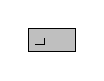
\begin{tikzpicture}[scale=0.3]
    \draw[thin,fill=lightgray] (0,0) rectangle (2,1);
    \draw (0.3,0.3) -- (0.7,0.3)--(0.7,0.6);     
\end{tikzpicture}}}

\definecolor{HIMAmuda}{HTML}{01D1FD}
\definecolor{HIMAtua}{HTML}{02016A}
\definecolor{HIMAabu}{HTML}{CBCBCC}
\definecolor{pgray}{rgb}{0.5,0.5,0.5}
\definecolor{pblue}{rgb}{0.13,0.13,1}
\definecolor{pgreen}{rgb}{0,0.5,0}
\definecolor{pred}{rgb}{0.9,0,0}
\definecolor{pgrey}{rgb}{0.46,0.45,0.48}
\definecolor{pcyan}{HTML}{D4EFFC}
\definecolor{lblue}{HTML}{00AEEF}
\definecolor{input}{HTML}{AAE1FA}
\definecolor{bg}{rgb}{0.95, 0.95, 0.92}
\definecolor{vscode}{HTML}{282A36}
\definecolor{PastelGreen}{HTML}{77DD77}

\newcommand{\inputscan}[1]{\raisebox{0pt}[1pt]{\colorbox{darkgray}{#1}}}

\usepackage{listings}

\lstdefinestyle{output}{
    language=Java,
    backgroundcolor=\color{vscode},
    basicstyle=\small\ttfamily\color{white},
    frame=none,
    escapeinside={(*}{*)},
    showspaces=false,
    showtabs=false,
    breaklines=true,
    showstringspaces=false,
    breakatwhitespace=true,
    keywordstyle=\color{white},
    }

\newtcblisting{RunCode}[1][enhanced,drop shadow]{
    arc=0pt, outer arc=0pt,
    boxsep=1pt,
    boxrule=2pt,
    auto outer arc,
    colback=vscode,
    colframe=bg,
    listing only, 
    listing style=output,
    title=\color{black}Ex. Output,
    #1
    }
\newtcblisting{RunCodeMore}[1][enhanced,drop shadow]{
    arc=0pt, outer arc=0pt,
    boxsep=1pt,
    boxrule=2pt,
    auto outer arc,
    colback=vscode,
    colframe=bg,
    listing only, 
    listing style=output,
    #1
    }

\newtcolorbox{hint}[1][]{
    colback=PastelGreen!5!white, 
    colframe=PastelGreen!75!black,
    fonttitle=\bfseries, 
    colbacktitle=PastelGreen!85!black,
    enhanced, 
    attach boxed title to top left={yshift=-2mm}, 
    title=Hint,
    before upper=\renewcommand\thempfootnote{\Roman{mpfootnote}},
    #1
}

\newtcolorbox{example}[1][]{
    colback=pgreen!5!white, 
    colframe=pgreen!75!black,
    fonttitle=\bfseries, 
    colbacktitle=pgreen!85!black,
    enhanced, 
    attach boxed title to top left={yshift=-2mm}, 
    title=Example,
    before upper=\renewcommand\thempfootnote{\Roman{mpfootnote}},
    #1
}

\newtcolorbox{req}[1][]{
    colback=lblue!5!white, 
    colframe=lblue!75!black,
    fonttitle=\bfseries, 
    colbacktitle=lblue!85!black,
    enhanced, 
    attach boxed title to top left={yshift=-2mm}, 
    title=Input,
    before upper=\renewcommand\thempfootnote{\Roman{mpfootnote}},
    #1
}

\newtcolorbox{out}[1][]{
    colback=HIMAtua!5!white, 
    colframe=HIMAtua!75!black,
    fonttitle=\bfseries, 
    colbacktitle=HIMAtua!85!black,
    enhanced, 
    attach boxed title to top left={yshift=-2mm}, 
    title=Output,
    before upper=\renewcommand\thempfootnote{\Roman{mpfootnote}},
    #1
}

\renewcommand{\thesubsection}{\arabic{subsection}}
\newcommand{\R}{\mathbb{R}}
\newcommand{\Z}{\mathbb{Z}}
\newcommand{\N}{\mathbb{N}}
\renewcommand{\figurename}{Gambar}

\floatstyle{ruled}
\newfloat{listing}{H}{lox}
\floatname{listing}{\strut Kode}

\setminted[java]{bgcolor=bg,fontsize=\small,bgcolorpadding=1mm,escapeinside=||,linenos,numbersep=5pt}

\title{\textbf{Week 5 Assigment}}
\date{28 April 2025}
\author{Teosofi H.A \& Hafidz M.}

\begin{document}
  \maketitle
  \pagenumbering{gobble}
  \section*{Tugas Mandiri}
  Buatlah class \texttt{Matriks2x2} yang merepresentasikan matriks berukuran $2\times 2$ dengan atribut \texttt{int a,b,c,d} dan beberapa method sebagai berikut:
  \begin{enumerate}
    \item \texttt{\color{blue}Matriks2x2(int a, int b, int c, int d)}: \textit{constructor} untuk menginisialisasi \texttt{Matriks2x2} dengan elemen \texttt{a,b,c,d}. Jika tidak ada parameter yang diberikan, maka inisialisasi dengan \texttt{0} untuk semua elemen.
    \[M_{2\times 2}=\begin{pmatrix} a & b \\ c & d \end{pmatrix}\]
    \item \texttt{\color{blue}multiply(Matriks2x2 m)}: method untuk mengalikan objek \texttt{Matriks2x2} dengan matriks lain \texttt{m} dan mengembalikan hasilnya dalam bentuk objek \texttt{Matriks2x2}.
    \item \texttt{\color{blue}trace()}: method untuk menghitung trace dari objek \texttt{Matriks2x2} dan mengembalikan hasilnya dalam bentuk integer.
    \[\text{Tr}(M)= a+d\]
    \item \texttt{\color{blue}determinan()}: method untuk menghitung determinan dari objek \texttt{Matriks2x2} dan mengembalikan hasilnya dalam bentuk integer.
    \[\det(M)= ad-bc\]
    \item \texttt{\color{blue}nilaiEigen()}: method untuk mencari semua nilai eigen dari objek \texttt{Matriks2x2} dan mengembalikan hasilnya dalam bentuk array.
    \[\lambda_{1,2}=\frac{\text{Tr}(M)\pm\sqrt{\text{Tr}(M)^2-4\det(M)}}{2}\]
    \item \texttt{\color{blue}printMatriks()}: method untuk mencetak objek \texttt{Matriks2x2} ke terminal.
  \end{enumerate}
  Selanjutnya, buatlah class \texttt{\color{red}Main} yang berisi method \texttt{main} untuk menguji class \texttt{Matriks2x2}. Buatlah objek \texttt{Matriks2x2} yang mempresentasikan matriks-matriks berikut:
  \begin{multicols}{3}
    \begin{itemize}
      \item $M_{1}=\begin{pmatrix} 1 & 2 \\ 3 & 4 \end{pmatrix}$
      \item $M_{2}=\begin{pmatrix} 1 & -3 \\ 3 & -5 \end{pmatrix}$
      \item $M_{3}=\begin{pmatrix} 2 & 1 \\ -5 & 2 \end{pmatrix}$
    \end{itemize}
  \end{multicols}
  \noindent Kemudian buatlah objek-objek untuk matriks hasil kali dari $M_{1}$, $M_{2}$, dan $M_{3}$. Terakhir, jalankan method-method pada objek-objek tersebut dan tampilkan hasilnya ke terminal.
  \begin{listing}[htbp]
  \begin{minted}{java}
class Matriks2x2 {
    public int a, b, c, d;
    public Matriks2x2() {
      //...
    }
    public Matriks2x2(int a, int b, int c, int d) {
      //...
    }
    
    public Matriks2x2 multiply(Matriks2x2 m) {
      //...
    }
    
    public int trace() {
      //...
    }
    
    public int determinan() {
      //...
    }
    
    public double[] nilaiEigen() {
      //...
    }

    public void printMatriks() {
      //...
    }
  }
  \end{minted}
  \caption{class Matriks2x2}
\end{listing}
  \begin{listing}[htbp]
  \begin{minted}{java}
class Main {
    public static void main(String[] args) {
      Matriks2x2 M1 = new Matriks2x2(1, 2, 3, 4);
      Matriks2x2 M2 = new Matriks2x2(1, -3, 3, -5);
      Matriks2x2 M3 = new Matriks2x2(2, 1, -5, 2);
      Matriks2x2 M4 = //...
      Matriks2x2 M5 = //...
      //...
    }
  }
  \end{minted}
  \caption{class Main}
\end{listing}
\end{document}